% IMPORTANT: add or remove (comment out) the boolean '\solutiontrue' below to
% create the solution document or the exercise document respectively.
% First we create the switch to make either the exercises or the solutions
\newif\ifsolution\solutionfalse
% To create the solution uncomment '\solutiontrue'
\solutiontrue

\documentclass[a4paper,11pt]{article}
\title{System Security,
\ifsolution Solution \else \fi
Reverse Engineering}

../author.tex

\usepackage[T1]{fontenc}
\usepackage{ae, aecompl}
\usepackage{a4wide}
\usepackage{boxedminipage}
\usepackage{url}
\usepackage{graphicx}
\usepackage{enumerate}
\usepackage{hyperref}
\usepackage{textcomp}
% Some useful commands and environments
\usepackage{framed}
\usepackage{listings}
\usepackage{ucs}
\usepackage[utf8x]{inputenc}
\usepackage[english]{babel}

\author{Andrei Pârvu}

\newenvironment{solution}%
{\par{\noindent\small\textit{Solution:}}\vspace{-12pt}\begin{framed}}%
{\end{framed}\par}


\begin{document}
\maketitle


\section*{Introduction}

In this assignment you will analyse the binary program {\tt challenge}.  You
find the it in the folder \texttt{disas}.  You will try to find a valid secret
for the binary program through Reverse Engineering. This will require reading
the disassembled binary. If you are not familiar with x86 assembly we recommend,
that you look at this guide:
\url{http://www.cs.virginia.edu/~evans/cs216/guides/x86.html} and read the
sections Registers, Addressing Memory and Size Directives. Additionally the
guide contains information on instructions you can use later.

To understand the problem, run the binary and test its behaviour. You will be
asked to enter a name as well as a secret. When entering the secret you might
encounter a message saying ``Wrong input format.''. Therefore your first task is
to understand how the secret input format should look like.

In general we recommend that you use gdb in this exercise. Using gdb can also
help you to discover the input format. Load the binary into gdb and
\verb|disassemble main| to see the disassembly. Initially it is easiest to look
for function calls, e.g. \verb|call   0x8048380 <puts@plt>|. To learn about the
puts function you can use the man pages by typing \verb|man 3 puts| into a
terminal. We see that puts expects a string as first parameter. To find the
string in the program, we see that the address 0x8048750 has been put on the top
of the stack (\verb|mov    DWORD PTR [esp],0x8048750|), so that 0x8048750 is the
first parameter. To print the string, we set a breakpoint at the call 
(\verb|b *0x080484de|), 
run the program and tell gdb to interpret the address as a string
\verb|x/s 0x8048750|. We find that this call prints the welcome string.
Similarly you can find the input format, by looking for a function that reads
user input.

After finding the correct input format, you can try it and should get an error
like ``Failed check 1.'' Apparently some checks are performed on the secret.
Try to understand the checks one after another. You can test your guess by
giving an input and stepping through the disassembly in gdb (\verb|ni|) and
seeing if you pass the check. To understand what ``passes'' you have to get an
idea, which control flow will lead you further. Therefore try to understand
where the ``Failed check 1.'' message is triggered and try to avoid this control
flow path.

As soon as you get the message ``Failed check 2.'' you have successfully passed
the first group of checks. The second check involves a loop. A loop typically
has a counter which is compared to another value and an backward jump that
depends on the comparison. A backward jump is one which jumps back to a
previously executed instruction.

Once you have passed all tests you should see a success message. Well done.


\section*{Expected Deliverables and Some Advice/Help}

First, we point out that this exercise is individual and we expect individual
submissions. Your submission should contain a brief explanation of some major
steps to summarize your findings.

\begin{enumerate}
\item What is the input format?
\item Briefly describe (e.g. in pseudo-code) what the first checks test?
\item What does the loop before the second check do?
\item Which were your successful inputs (name and secret)?
\end{enumerate}

\ifsolution
\begin{solution}
First of all, the input name has to have a length higher or equal than four (there
is a clear message which states this). After entering the name, I entered the secret
(just a simple number) and obtained \texttt{Wrong input format.}. To check why this
happens, I disassembled the program and checked for the code which reads the secret
(I looked for a call to \texttt{scanf} or something similar). After finding it, I
discovered that the return value of scanf (which is stored in \texttt{[ebp-0x10]})
had to be $4$. In this case I had to check the format string of scanf, which is
located at \texttt{0x80487cb} and saw that it is \texttt{"\%u-\%u-\%u-\%u"}, so I
had to provide $4$ numbers separated by hyphens.\\
After entering the secret in this format, I received \texttt{Failed check 1}. I continued
to investigate the assembly code and I found that 5 different constraints were verified:
\begin{enumerate}
  \item The first input, stored at \texttt{[ebp-0x60]} is compared to the hexa number
  \texttt{0xdeadf00d}. Thus, the first number of the secret has to be $3735941133$, in base $10$.
  \item The second input is checked to be equal to the double word that is formed from the input
  string. Because I entered \texttt{andrei} and the numbering format is little-endian this conversion
  was equal to $'r' * (2 ^{24}) + 'd' * (2^{16}) + 'n' * (2^{8}) + 'a'$. This is why the length of the
  name has to be at least $4$.
  \item The third input is checked to have the third most significant byte equal to \texttt{0x2a}.
  \item The sum of the fourth and third most significant byte of the third input has to be equal
  to the second most significant byte
  \item The most significant byte of the third input has to be equal to \texttt{0x17}.
\end{enumerate}

In pseudocode, this first check is:
\begin{lstlisting}
  if (input1 != 0xdeadf00d) {
    fail1_and_exit();
  }
  if (*(int*)name != input2) {
    fail1_and_exit();
  }
  if ((input3 >> 8)) & 0xff != 0x2a) {
    fail1_and_exit();
  }
  if ((input3 & 0xff) + ((input3 >> 8) & 0xff) !=
      (input3 >> 16) & 0xff) {
    fail1_and_exit();
  }
  if ((input3 >> 24) & 0xff != 0x17) {
    fail1_and_exit();
  }
\end{lstlisting}

  The second check performs a loop through all the characters of the provided name. The counter
  is stored in \texttt{[ebp-0x8]}, and each time the loop is executed it gets compared to the length
  of the name (which is stored in \texttt{eax}). During the loop the bytes that form the name string
  get added and their sum is stored in \texttt{ebp-0xc}. At the end, this sum is multiplied by \texttt{0x2a}
  and compared to the fourth element of the secret. If it is equal a success message is displayed.\\

  In conclusion, the particular input that I used was the string \texttt{"andrei"} for the name and
  the secret \texttt{3735941133-1919184481-388639232-26334}. This execution can be seen in Figure~\ref{fig:exe}.

\end{solution}\fi

\begin{figure} \center
  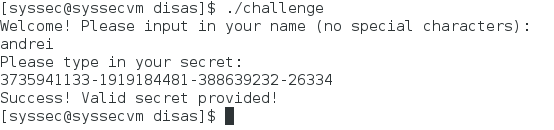
\includegraphics[width=0.8\linewidth]{disas.png}
  \caption{Execution}
  \label{fig:exe}
\end{figure}

\end{document}
